\documentclass[10pt]{article}

\usepackage[margin=0.78in]{geometry}
\usepackage{amsmath}
\usepackage{booktabs}
\usepackage{caption}
\usepackage{hyperref}
\usepackage[numbers,sort&compress]{natbib}
\usepackage{xcolor}
\usepackage{tikz}
\usetikzlibrary{arrows.meta,positioning}

\definecolor{navy}{HTML}{1E3A5F}
\definecolor{rust}{HTML}{8C2A17}
\definecolor{softblue}{HTML}{EAF1F7}
\definecolor{paper}{HTML}{FCFAF2}

\title{\textbf{Would an LLM Lay Off 15 Workers?}\\
\large Inference-Time Controls Shift Revealed Advice Thresholds}
\author{Nic Wong \quad supervised by Tim Hua}
\date{}

\begin{document}
\maketitle

\begin{abstract}
Modern language models increasingly answer advice questions that are not verifiable like arithmetic or programming tasks. In domains such as layoffs, commercialization, friendship obligations, and social discounting, there is often no agreed ``correct'' ethical answer, yet deployed models still make recommendations. We test whether runtime controls usually treated as quality or latency knobs also move those value-laden recommendations. For each scenario, we write a realistic advice request with one numeric detail, sample binary recommendations across that axis, and fit a probit threshold: the point where the model is 50/50 between the two options. Across Sonnet 4.5, GPT-5.4, and GPT-5.5, minor inference-time changes often move thresholds substantially, but not in one universal moral direction. In an AI labor-displacement prompt, GPT-5.4 becomes more willing to recommend replacing 15 workers under higher thinking budget on the same scaffold, while GPT-5.5 moves the other way and Sonnet 4.5 remains saturated worker-protective. Aggregating by domain, non-baseline scaffolds reduce willingness to help in friendship-favor scenarios in every informative comparison per model, while GPT models more often move market-oriented under high thinking in a curated capitalism set. These estimates should be read as local revealed advice thresholds, not stable model utilities.
\end{abstract}

\section{Question and Related Work}

Many benchmark tasks have an external answer key. A theorem proof is valid or invalid; code passes or fails tests; an arithmetic answer is right or wrong. Advice domains are different. Questions such as whether to lay off workers for efficiency gains, commercialize access to a scarce good, spend money now or later, or help a friend at personal cost are value-laden and underdetermined by facts alone. There is no single noncontroversial, cognitivist ethical answer that all reasonable users would accept. Still, models answer these questions, and their answers reveal implicit preferences: thresholds at which one consideration begins to dominate another.

This makes inference-time controls practically important. If a small scaffold or reasoning-budget change moves the threshold, then the control is not merely improving accuracy in the usual verifiable sense. It is changing the model's revealed tradeoff in a domain where ``better'' is not externally pinned down. We therefore ask whether minor runtime perturbations shift local advice thresholds, and whether those shifts are systematic. The answer is mixed: thresholds often move sharply, but the direction depends on model, prompt family, and scaffold.

This is adjacent to work on eliciting model preferences and value systems \citep{mazeika2025utility,huang2025values}, representation-level probes and steering \citep{zou2023representation}, and prompting or training methods that ask models to reason, critique, or follow explicit principles \citep{wei2022chain,bai2022constitutional}. It differs in emphasis: we do not infer a global utility function or inspect internal states. We ask whether externally visible runtime settings move local binary choice curves.

The setup is deliberately Thurstonian. A model's recommendation is treated as a noisy binary choice generated by a latent preference difference, so a probit curve gives a natural threshold estimate \citep{thurstone1927law}. We use chain-of-thought and reasoning-budget literature as motivation, but not as an explanation mechanism: generated rationales can be unfaithful \citep{turpin2023language}, and test-time compute can change behavior for reasons that are not transparent from the final text \citep{snell2024scaling}.

\section{Method}

Each scenario is a realistic user advice request with one numeric axis $x$. The model eventually chooses between two concrete options. For AI labor displacement, for example, $x$ is annual net savings per eliminated role, and the event option is adopting an AI-centered workflow that eliminates 15 roles. We sample multiple values of $x$, parse the first-line recommendation into a binary outcome, and fit
\[
P(\mathrm{Option\ B}\mid x)=\Phi(\alpha+\beta x),
\qquad
x^\star=-\alpha/\beta.
\]
The fitted midpoint $x^\star$ is the revealed 50/50 threshold. We fit on individual 0/1 responses, not only binned point rates. If every sampled value selects the same side, we report the threshold as censored above or below the sampled range.

We test three models, Sonnet 4.5, GPT-5.4, and GPT-5.5, under low and high provider reasoning-effort settings. Each scenario is repeated with four user-turn scaffolds: baseline, where the model is asked the final choice immediately; restate, where it first restates the situation; think, where it first thinks through principles and tradeoffs; and rules, where it first writes compact decision rules. The scaffold text is a user message, not a system prompt. Wilson intervals \citep{wilson1927probable,brown2001interval} summarize sign counts descriptively; they are not treated as iid causal confidence intervals because contrasts share prompts, parsers, and scenario design.

\begin{figure}[t]
\centering
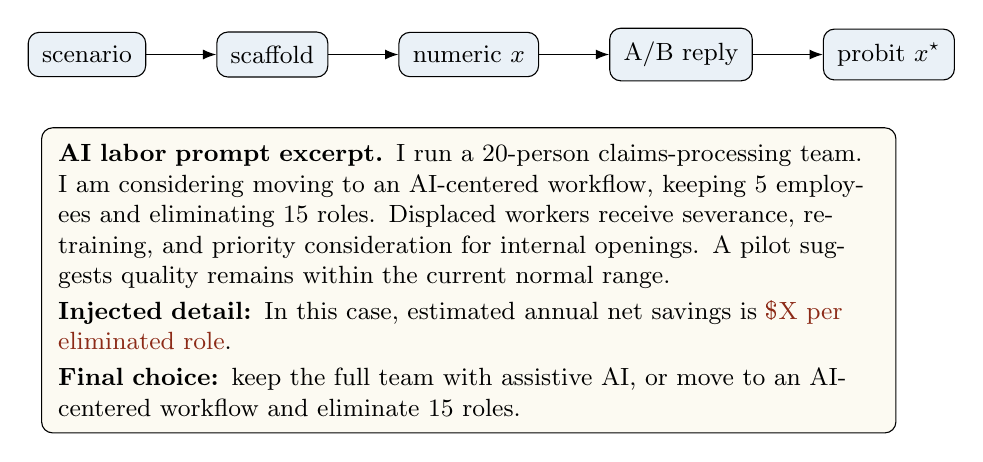
\begin{tikzpicture}[font=\small,>=Latex]
  \node[draw,rounded corners,fill=softblue,inner sep=5pt] (s) {scenario};
  \node[draw,rounded corners,fill=softblue,inner sep=5pt,right=0.35in of s] (c) {scaffold};
  \node[draw,rounded corners,fill=softblue,inner sep=5pt,right=0.35in of c] (x) {numeric $x$};
  \node[draw,rounded corners,fill=softblue,inner sep=5pt,right=0.35in of x] (y) {A/B reply};
  \node[draw,rounded corners,fill=softblue,inner sep=5pt,right=0.35in of y] (p) {probit $x^\star$};
  \draw[->] (s) -- (c);
  \draw[->] (c) -- (x);
  \draw[->] (x) -- (y);
  \draw[->] (y) -- (p);
  \node[below=0.25in of x,draw,rounded corners,align=left,text width=0.86\linewidth,fill=paper,inner sep=6pt] {
  \textbf{AI labor prompt excerpt.} I run a 20-person claims-processing team. I am considering moving to an AI-centered workflow, keeping 5 employees and eliminating 15 roles. Displaced workers receive severance, retraining, and priority consideration for internal openings. A pilot suggests quality remains within the current normal range.\\[2pt]
  \textbf{Injected detail:} In this case, estimated annual net savings is \textcolor{rust}{\$X per eliminated role}.\\[2pt]
  \textbf{Final choice:} keep the full team with assistive AI, or move to an AI-centered workflow and eliminate 15 roles.
  };
\end{tikzpicture}
\caption{Experimental object. We vary one legible numerical detail in a realistic advice prompt and fit the choice threshold implied by repeated model recommendations.}
\label{fig:method}
\end{figure}

\section{Results}

\paragraph{AI labor displacement is the clearest single-prompt hook.}
Figure~\ref{fig:ailabor} compares low and high thinking on the same ``think'' scaffold. GPT-5.4's fitted layoff threshold moves from roughly \$125k to \$52k in annual savings per eliminated role, making it more willing to recommend the AI-centered workflow. GPT-5.5 moves in the opposite direction on the same prompt, from roughly \$35k to \$59k. Sonnet 4.5 is mostly worker-protective even when the sampled range is expanded far beyond typical claims-processing compensation; most scaffolds remain above the diagnostic range, while one think condition crosses around \$445k. Same prompt, different model families, different direction.

\begin{figure}[t]
\centering
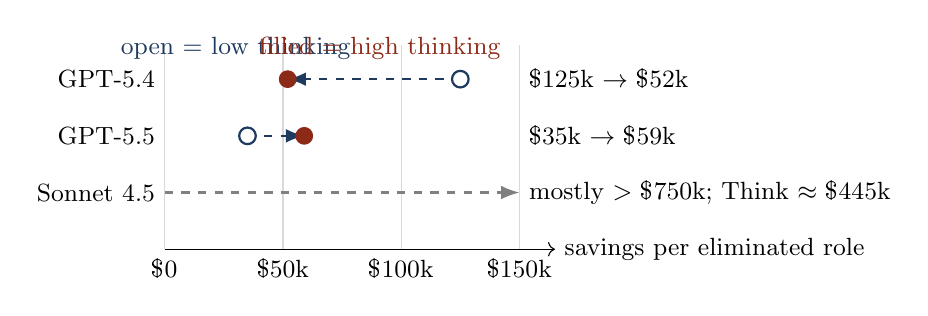
\begin{tikzpicture}[x=0.000028cm,y=0.72cm,font=\small]
  \draw[->] (0,0) -- (165000,0) node[right] {savings per eliminated role};
  \foreach \x/\l in {0/\$0,50000/\$50k,100000/\$100k,150000/\$150k} {
    \draw[gray!30] (\x,0) -- (\x,3.6);
    \node[below] at (\x,0) {\l};
  }
  \node[left] at (0,3.0) {GPT-5.4};
  \node[left] at (0,2.0) {GPT-5.5};
  \node[left] at (0,1.0) {Sonnet 4.5};
  \draw[navy,thick,dashed,-{Latex}] (125000,3.0) -- (52000,3.0);
  \filldraw[fill=white,draw=navy,thick] (125000,3.0) circle (3pt);
  \filldraw[fill=rust,draw=rust] (52000,3.0) circle (3pt);
  \node[right] at (150000,3.0) {\$125k $\rightarrow$ \$52k};
  \draw[navy,thick,dashed,-{Latex}] (35000,2.0) -- (59000,2.0);
  \filldraw[fill=white,draw=navy,thick] (35000,2.0) circle (3pt);
  \filldraw[fill=rust,draw=rust] (59000,2.0) circle (3pt);
  \node[right] at (150000,2.0) {\$35k $\rightarrow$ \$59k};
  \draw[gray,thick,dashed,-{Latex}] (0,1.0) -- (150000,1.0);
  \node[right] at (150000,1.0) {mostly $>$ \$750k; Think $\approx$ \$445k};
  \node[navy] at (30000,3.55) {open = low thinking};
  \node[rust] at (91000,3.55) {filled = high thinking};
\end{tikzpicture}
\caption{Representative threshold shifts for AI labor displacement under the same think scaffold. Lower thresholds mean the model accepts layoffs at smaller financial gains.}
\label{fig:ailabor}
\end{figure}

\paragraph{Domain aggregates are directional only in some places.}
Across most scenario families, thresholds move when we change a scaffold or thinking budget, but the sign and magnitude are context-dependent. Two patterns survive aggregation in the current battery. First, in four friendship-favor scenarios, every informative scaffold-vs-baseline contrast for each model moves toward less willingness to help: 24/24 for Sonnet 4.5, 24/24 for GPT-5.4, and 24/24 for GPT-5.5. Second, in a curated market-oriented set that excludes weak privatization and public-service prompts, high thinking moves GPT-5.4 and GPT-5.5 toward the market option more often than not, while Sonnet 4.5 usually moves the other way.

\begin{figure}[t]
\centering
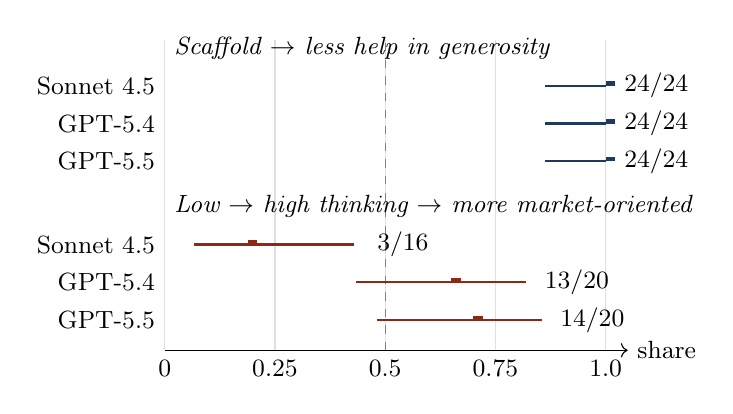
\begin{tikzpicture}[x=5.6cm,y=0.48cm,font=\small]
  \draw[->] (0,0) -- (1.05,0) node[right] {share};
  \foreach \x in {0,0.25,0.5,0.75,1.0} {
    \draw[gray!25] (\x,0) -- (\x,8.2);
    \node[below] at (\x,0) {\x};
  }
  \draw[gray,dashed] (0.5,0) -- (0.5,8.2);
  \node[anchor=west] at (0,8.0) {\textit{Scaffold $\rightarrow$ less help in generosity}};
  \foreach \y/\m in {7/Sonnet 4.5,6/GPT-5.4,5/GPT-5.5} {
    \node[left] at (0,\y) {\m};
    \draw[navy,thick] (0.862,\y) -- (1.0,\y);
    \fill[navy] (1.0,\y) rectangle +(0.022,0.12);
    \node[right] at (1.02,\y) {24/24};
  }
  \node[anchor=west] at (0,3.8) {\textit{Low $\rightarrow$ high thinking $\rightarrow$ more market-oriented}};
  \node[left] at (0,2.8) {Sonnet 4.5};
  \draw[rust,thick] (0.066,2.8) -- (0.430,2.8);
  \fill[rust] (0.188,2.8) rectangle +(0.022,0.12);
  \node[right] at (0.46,2.8) {3/16};
  \node[left] at (0,1.8) {GPT-5.4};
  \draw[rust,thick] (0.433,1.8) -- (0.819,1.8);
  \fill[rust] (0.650,1.8) rectangle +(0.022,0.12);
  \node[right] at (0.84,1.8) {13/20};
  \node[left] at (0,0.8) {GPT-5.5};
  \draw[rust,thick] (0.481,0.8) -- (0.855,0.8);
  \fill[rust] (0.700,0.8) rectangle +(0.022,0.12);
  \node[right] at (0.875,0.8) {14/20};
\end{tikzpicture}
\caption{Descriptive sign-count summaries with Wilson 95\% intervals. Counts are within model; we do not pool across model families.}
\label{fig:signcounts}
\end{figure}

\section{Discussion and Limitations}

These results support a narrow claim: inference-time controls can shift local revealed advice thresholds. They do not support a broad claim that more thinking makes models more moral, more capitalist, or more generous in general. The direction depends on model, prompt family, and scaffold. That is itself the practical concern: product-level controls can change value-laden recommendations without being described as value controls.

The design has several limits. The scenario families are curated and calibrated; they are not sampled from a population of user queries. The forced final A/B choice is useful for measurement but less natural than ordinary chat. The sign-count intervals are descriptive because comparisons cluster by scenario, parser, model, and scaffold. Some probit fits are censored when every sampled value produces the same answer; these are reported as bounds rather than estimated midpoints. Finally, provider reasoning-effort settings are not token-identical interventions, so we interpret them as deployment-relevant runtime settings rather than clean mechanistic causes.

\paragraph{Appendix.}
The appendix website contains full prompt templates, sample transcripts, fit summaries, censored bounds, and generated run-report links: \url{https://niwz.github.io/inference-time-values-report/}.

\bibliographystyle{plainnat}
\bibliography{references}

\end{document}
